\chapter{NFC Chip Configuration and libnfc Setup}
\label{app:nfc-chip-config}

To make the Raspberry Pi serially communicate with the NF Chip, the `SEL1'
pads were shorted (see Fig.
\ref{fig:nfc-chip-solder}). With this done, the chip can serially communicate
with the Raspberry Pi's UART interface.

\begin{figure}
 \centering 
 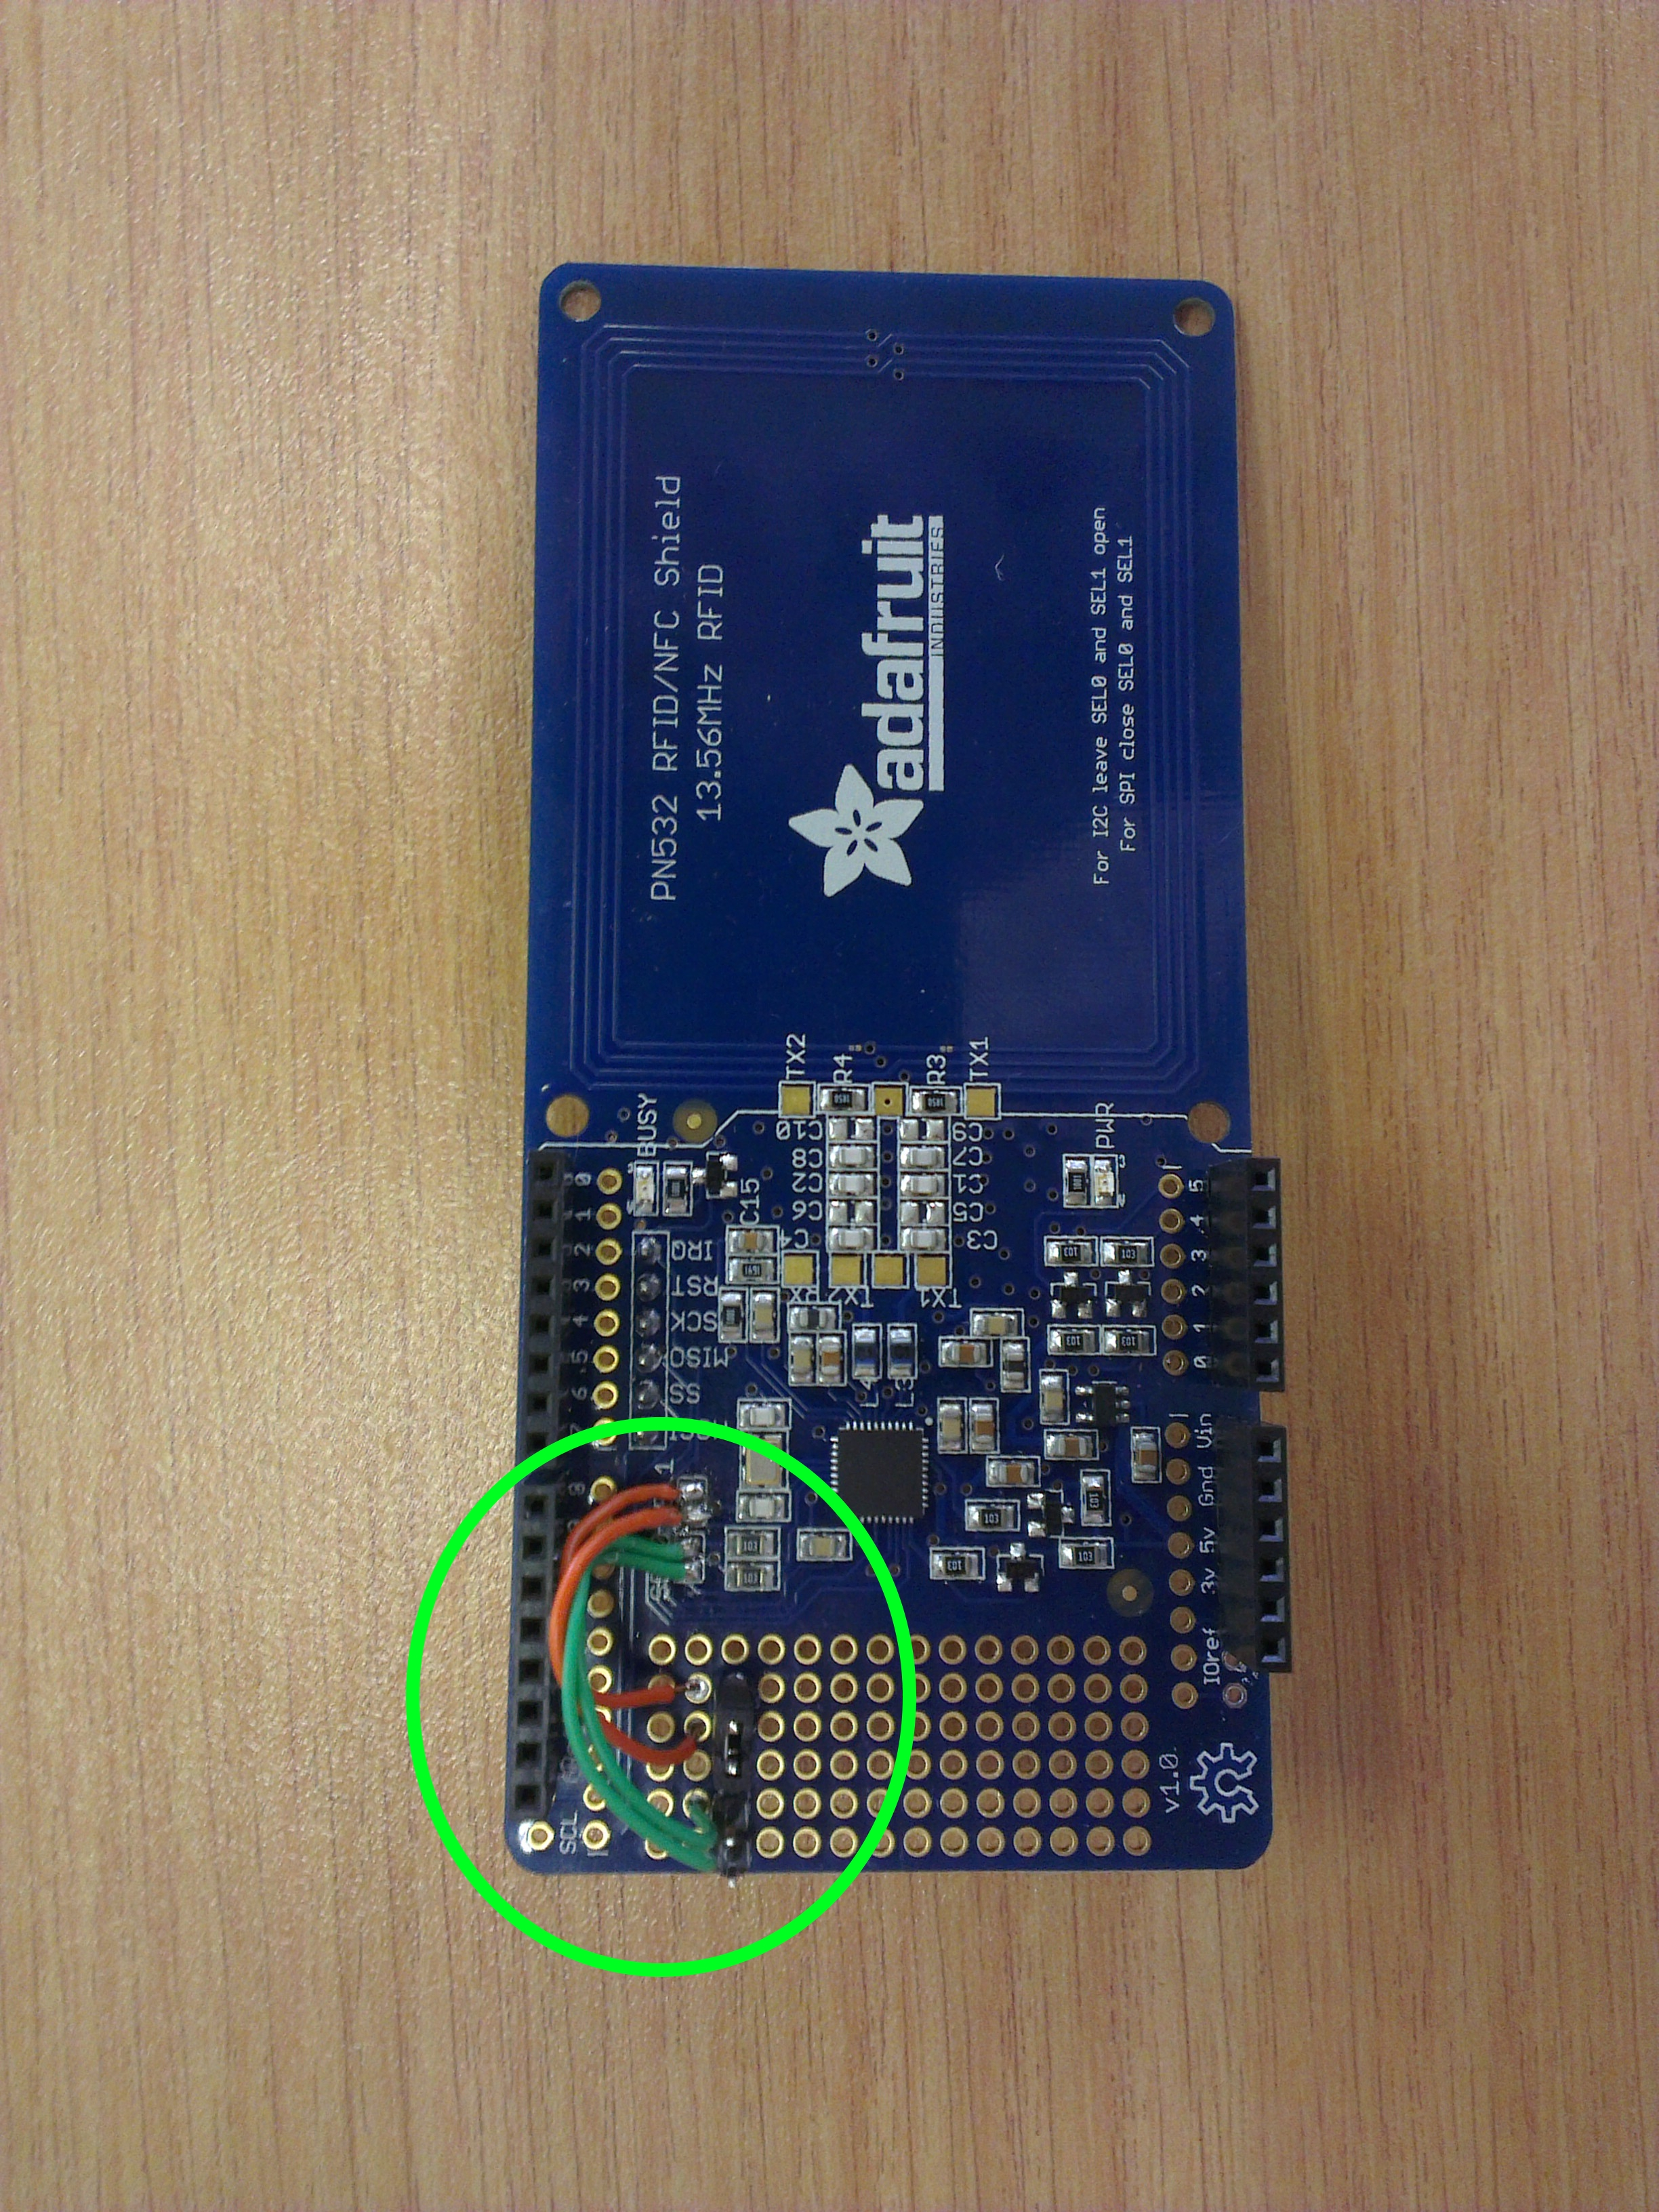
\includegraphics[clip=true, trim = 0 250 0 290,
 scale=0.1]{soldeer_pic}
 \caption[The location of the SEL1 pads.]{The location of the SEL1 pads (circled
 in green).}
 \label{fig:nfc-chip-solder}
\end{figure}

The connections between the Pi and the NFC controller are given in Table
\ref{tab:chip-connections}.

\begin{table}
\centering
 \caption{Connections between the Raspberry Pi and the NFC Controller chip.}
 \begin{tabular}{|l|l|l|}
  \hline
  \textbf{NCF Controller Pin} & \textbf{Raspberry Pi Pin}\\\hline\hline
  5V pin & 5V (pin 4) \\\hline
  Ground pin & Ground pin (pin 6) \\\hline
  SS & UART0 TXD (pin 8) \\\hline
  MOSI & UART0 RXD (pin 10) \\\hline
 \end{tabular}
 \label{tab:chip-connections}
\end{table}

\section{libnfc Setup on the Raspberry Pi}

Before libnfc could be built and configured, a communication line between the NFC
controller and the Pi needed to be opened. To do this, the Pi's UART needed
to be freed up. By default, the Raspberry Pi uses its UART to serially write out
its booting information. Therefore, to allow the Raspberry Pi to communicate
with the NFC controller via its UART0 interface, it was necessary to modify
some of its configuration files. To do this, the Adafruit tutorial was followed
[\cite{website:adafruit-tutorial}].

The file `/boot/cmdline.txt' and `/etc/inittab' had to be edited to
contain the following lines of code:

\textbf{cmdline.txt}
\begin{verbatim}
dwc_otg.lpm_enable=0 console=tty1
\end{verbatim}

\textbf{inittab}
\begin{verbatim}
#Spawn a getty on Raspberry Pi serial line
#T0:23:respawn:/sbin/getty -L ttyAMA0 115200 vt100
\end{verbatim}

After this was done, the libnfc package could be configured and installed 
to work with the Pi's UART interface.

Thereafter, the Pi was ready to receive NFC messages from the NFC shield.